\chapter{System Implementation}
\label{chapter:SystemImplementation}
%\TODO{In this chapter, we will describe in detail the implementation of both server and client of our mesh streaming framework.}
We have describe the design of our mesh streaming system in the previous chapter. In this chapter, we will describe the implementation details of our system both in server and client side. 
\begin{figure}[htb]
	\centering
	
	\begin{pdfpic}
	\psset{unit=0.90cm}
	\begin{pspicture}
	\psframe[linewidth=0.1,dimen=outer](2.8,6.44)(0.4,5.52)
\usefont{T1}{ptm}{m}{n}
\rput(1.5690235,5.985){Server Start}
\psframe[linewidth=0.1,dimen=outer](8.7,6.4)(6.28,5.48)
\usefont{T1}{ptm}{m}{n}
\rput(7.4237695,5.945){Client Start}
\psframe[linewidth=0.1,dimen=outer](5.7,4.9)(3.26,3.98)
\usefont{T1}{ptm}{m}{n}
\rput(4.4737697,4.445){Connect}
\psdiamond[linewidth=0.1,dimen=outer](4.5,0.96)(2.1,0.9)
\usefont{T1}{ptm}{m}{n}
\rput(4.4314356,0.965){Server Rendering?}
\psframe[linewidth=0.1,dimen=outer](2.8,-0.1)(0.0,-1.02)
\psline[linewidth=0.1,arrowsize=0.05291667cm 2.0,arrowlength=1.4,arrowinset=0.4]{->}(2.5,0.96)(1.4,0.96)(1.4,-0.14)
\psframe[linewidth=0.1,dimen=outer](5.7,3.3)(3.26,2.38)
\usefont{T1}{ptm}{m}{n}
\rput(4.5250683,2.845){Select Model}
\psline[linewidth=0.1cm,arrowsize=0.05291667cm 2.0,arrowlength=1.4,arrowinset=0.4]{->}(4.5,2.46)(4.5,1.86)
\psline[linewidth=0.1cm,arrowsize=0.05291667cm 2.0,arrowlength=1.4,arrowinset=0.4]{->}(4.52,4.06)(4.52,3.28)
\psline[linewidth=0.1,arrowsize=0.05291667cm 2.0,arrowlength=1.4,arrowinset=0.4]{->}(6.5,0.96)(7.7,0.96)(7.7,-0.14)
\usefont{T1}{ptm}{m}{n}
\rput(2.3161328,1.165){No}
\usefont{T1}{ptm}{m}{n}
\rput(6.772051,1.165){Yes}
\psframe[linewidth=0.1,dimen=outer](9.1,-0.1)(6.3,-1.14)
\usefont{T1}{ptm}{m}{n}
\rput(1.3978711,-0.535){Receive $vsplit$}
\psframe[linewidth=0.1,dimen=outer](2.8,-1.7)(0.0,-2.62)
\psline[linewidth=0.1cm,arrowsize=0.05291667cm 2.0,arrowlength=1.4,arrowinset=0.4]{->}(1.4,-0.94)(1.4,-1.74)
\usefont{T1}{ptm}{m}{n}
\rput(1.3872851,-2.135){Mesh Refinement}
\usefont{T1}{ptm}{m}{n}
\rput(4.5835447,-2.335){Synchronize}
\psframe[linewidth=0.1,dimen=outer](2.8,-3.1)(0.0,-4.02)
\psline[linewidth=0.1cm,arrowsize=0.05291667cm 2.0,arrowlength=1.4,arrowinset=0.4]{->}(1.4,-2.54)(1.4,-3.14)
\usefont{T1}{ptm}{m}{n}
\rput(1.3436719,-3.535){Rendering}
\usefont{T1}{ptm}{m}{n}
\rput(7.6717186,-0.435){Receive}
\usefont{T1}{ptm}{m}{n}
\rput(7.681719,-0.835){Rendered Image}
\psframe[linewidth=0.1,dimen=outer](9.1,-1.9)(6.3,-2.82)
\psline[linewidth=0.1cm,arrowsize=0.05291667cm 2.0,arrowlength=1.4,arrowinset=0.4]{->}(7.7,-1.04)(7.7,-1.94)
\usefont{T1}{ptm}{m}{n}
\rput(7.655869,-2.335){Display}
\usefont{T1}{ptm}{m}{n}
\rput(4.592139,-2.635){Viewing Params}
\psline[linewidth=0.04cm,arrowsize=0.05291667cm 2.0,arrowlength=1.4,arrowinset=0.4]{<-}(3.4,-1.14)(4.4,-2.04)
\psline[linewidth=0.04cm,arrowsize=0.05291667cm 2.0,arrowlength=1.4,arrowinset=0.4]{<-}(5.7,-1.14)(4.7,-2.04)
\psline[linewidth=0.1,arrowsize=0.05291667cm 2.0,arrowlength=1.4,arrowinset=0.4]{->}(1.4,-3.94)(1.4,-4.34)(3.2,-4.34)(3.2,0.36)(1.4,0.36)
\psline[linewidth=0.1,arrowsize=0.05291667cm 2.0,arrowlength=1.4,arrowinset=0.4]{->}(7.7,-2.7557895)(7.7,-3.34)(6.0,-3.34)(6.0,0.36)(7.7,0.36)
\psframe[linewidth=0.1,dimen=outer](6.2,-5.54)(2.8,-6.44)
\psline[linewidth=0.1,arrowsize=0.05291667cm 2.0,arrowlength=1.4,arrowinset=0.4]{->}(1.4,-4.34)(1.4,-5.04)(4.5,-5.04)(4.5,-5.54)
\psline[linewidth=0.1](7.7,-3.34)(7.7,-5.04)(4.5,-5.04)
\usefont{T1}{ptm}{m}{n}
\rput(4.478291,-5.935){Connection Close}
\psline[linewidth=0.1,arrowsize=0.05291667cm 2.0,arrowlength=1.4,arrowinset=0.4]{->}(2.7,5.96)(4.5,5.96)(4.5,4.86)
\psline[linewidth=0.1,arrowsize=0.05291667cm 2.0,arrowlength=1.4,arrowinset=0.4]{->}(6.3,5.96)(4.5,5.96)(4.5,4.86)
	\end{pspicture}
	\end{pdfpic} 
	\caption{Overall Process Flow Chart}
	\label{fig:flowchart}

\end{figure}
To describe the implementation of our streaming system, let's first take a look at the flow char of overall process \FG{fig:flowchart} shows. Consider a user is using our streaming system to view a mesh model progressively, the process goes as follows: 
\begin{enumerate}
\item
Client/Server start and connect. 
\item
Select a model to view.
\item
If not using server rendering, continuously receiving $vsplits$ transmitted from server based on synchronized viewing parameter. And then perform mesh refinement and rendering.
\item
If using server rendering, continuously receiving rendered images from server based on synchronized viewing parameters.
\item
Connection closes.
\end{enumerate}
\FG{fig:flowchart} illustrates the functionalities of our streaming system out of the box. In the following sections we will describe the implementation details of each steps illustrated in \FG{fig:flowchart}. 

\section{Model Loading}
\label{section:modelloading}
Both of the client and server have the functionality of model loading. The server need to load a view-dependent progressive mesh model when a a user selects it from client-side. And vice versa, the client also need to load the bash mesh of the selected model transmitted from server. Therefore, in this section, we will describe in detail the file format of the view-dependent progressive mesh model. \\
%\subsection{File Format} 
%\label{section:fileformat}
\begin{figure}[htb]
	\centering
	
	\begin{pdfpic}
\psframe[linewidth=0.1,dimen=outer](5.5,3.95)(0.4,3.35)
\usefont{T1}{ptm}{m}{n}
\rput(3.018, 3.655){Header}
\psframe[linewidth=0.1,dimen=outer](5.5,3.45)(0.4,2.85)
\usefont{T1}{ptm}{m}{n}
\rput(3.018, 3.155){Number of base vertices $n_v$}
\psframe[linewidth=0.1,dimen=outer](5.5,2.95)(0.4,2.35)
\usefont{T1}{ptm}{m}{n}
\rput(3.018, 2.655){Number of base faces $n_f$}
\psframe[linewidth=0.1,dimen=outer](5.5,2.45)(0.4,1.85)
\usefont{T1}{ptm}{m}{n}
\rput(3.018, 2.155){Number of Details $n_d$}
\psframe[linewidth=0.1,dimen=outer](5.5,-2.05)(0.4,-2.65)
\usefont{T1}{ptm}{m}{n}
\rput(3.018, -2.345){Detail $d_1$}
\usefont{T1}{ptm}{m}{n}
\rput{-90.0}(6.0606833,-0.1906836){\rput(2.8925195,-2.975){\LARGE ...}}
\psframe[linewidth=0.1,dimen=outer](5.5,-3.55)(0.4,-4.15)
\usefont{T1}{ptm}{m}{n}
\rput(3.018,-3.845){Detail $d_{n_d}$}
\psframe[linewidth=0.1,dimen=outer](5.5,1.95)(0.4,1.35)
\usefont{T1}{ptm}{m}{n}
\rput(3.018, 1.655){Base vertex $v_1$}
\usefont{T1}{ptm}{m}{n}
\rput{-90.0}(2.0606835,3.8093164){\rput(2.8925195,1.025){\LARGE ...}}
\psframe[linewidth=0.1,dimen=outer](5.5,0.45)(0.4,-0.15)
\usefont{T1}{ptm}{m}{n}
\rput(3.018, 0.155){Base vertex $v_{n_v}$}
\psframe[linewidth=0.1,dimen=outer](5.5,-0.05)(0.4,-0.65)
\usefont{T1}{ptm}{m}{n}
\rput(3.018, -0.345){Base face $f_1$}
\psframe[linewidth=0.1,dimen=outer](5.5,-1.55)(0.4,-2.15)
\usefont{T1}{ptm}{m}{n}
\rput(3.018, -1.845){Base vertex $v_{n_f}$}
\usefont{T1}{ptm}{m}{n}
\rput{-90.0}(4.0606833,1.8093164){\rput(2.8925195,-0.975){\LARGE ...}}
\usefont{T1}{ptm}{m}{n}
\rput(3.0118067,4.255){Progressive Mesh File}
\pspolygon[linewidth=0.1](0.0,4.65)(0.0,-4.65)(5.9,-4.65)(5.9,4.15)(5.113333,4.65)
\psline[linewidth=0.1](5.1,4.65)(5.1,4.15)(5.9,4.15)
	\end{pdfpic} 
	\caption{Simple Progressive Mesh File Format}
	\label{fig:pmfileformat}

\end{figure}
\begin{figure}[htb]
	\centering
	
	\begin{pdfpic}
	\psframe[linewidth=0.1,dimen=outer](5.5,3.65)(0.4,3.05)
\usefont{T1}{ptm}{m}{n}
\rput(3.018, 3.355){Header}
\psframe[linewidth=0.1,dimen=outer](5.5,3.15)(0.4,2.55)
\usefont{T1}{ptm}{m}{n}
\rput(3.018, 2.855){Number of base vertices $n_v$}
\psframe[linewidth=0.1,dimen=outer](5.5,2.65)(0.4,2.05)
\usefont{T1}{ptm}{m}{n}
\rput(3.018, 2.355){Number of base faces $n_f$}
\psframe[linewidth=0.1,dimen=outer](5.5,2.15)(0.4,1.55)
\usefont{T1}{ptm}{m}{n}
\rput(3.018, 1.855){Number of Details $n_d$}
\psframe[linewidth=0.1,dimen=outer](5.5,1.65)(0.4,1.05)
\usefont{T1}{ptm}{m}{n}
\rput(3.018, 1.355){Base vertex $v_1$}
\usefont{T1}{ptm}{m}{n}
\rput{-90.0}(2.3606834,3.5093164){\rput(2.8925195,0.725){\LARGE ...}}
\psframe[linewidth=0.1,dimen=outer](5.5,0.15)(0.4,-0.45)
\usefont{T1}{ptm}{m}{n}
\rput(3.018, -0.145){Base vertex $v_{n_v}$}
\psframe[linewidth=0.1,dimen=outer](5.5,-0.35)(0.4,-0.95)
\usefont{T1}{ptm}{m}{n}
\rput(3.018, -0.645){Base face $f_1$}
\psframe[linewidth=0.1,dimen=outer](5.5,-1.85)(0.4,-2.45)
\usefont{T1}{ptm}{m}{n}
\rput(3.018, -2.145){Base face $f_{n_f}$}
\usefont{T1}{ptm}{m}{n}
\rput{-90.0}(4.3606834,1.5093163){\rput(2.8925195,-1.275){\LARGE ...}}
\usefont{T1}{ptm}{m}{n}
\rput(2.923213,3.955){View-dependent PM File}
\pspolygon[linewidth=0.1](0.0,4.35)(0.0,-4.35)(5.9,-4.35)(5.9,3.8822582)(5.113333,4.35)
\psline[linewidth=0.1](5.1,4.35)(5.1,3.85)(5.9,3.85)
\psline[linewidth=0.04cm](1.3,-2.55)(1.3,-2.85)
\psline[linewidth=0.04](0.9,-3.05)(0.9,-2.85)(1.7,-2.85)(1.7,-3.05)
\psline[linewidth=0.04](0.7,-3.25)(0.7,-3.05)(1.1,-3.05)(1.1,-3.25)
\psline[linewidth=0.04](1.5,-3.25)(1.5,-3.05)(1.9,-3.05)(1.9,-3.25)
\psline[linewidth=0.04](0.6,-3.45)(0.6,-3.25)(0.8,-3.25)(0.8,-3.45)
\psline[linewidth=0.04](1.0,-3.45)(1.0,-3.25)(1.2,-3.25)(1.2,-3.45)
\psline[linewidth=0.04](1.4,-3.45)(1.4,-3.25)(1.6,-3.25)(1.6,-3.45)
\psline[linewidth=0.04](1.8,-3.45)(1.8,-3.25)(2.0,-3.25)(2.0,-3.45)
\psline[linewidth=0.04cm](2.9,-2.55)(2.9,-2.85)
\psline[linewidth=0.04](2.5,-3.05)(2.5,-2.85)(3.3,-2.85)(3.3,-3.05)
\psline[linewidth=0.04](2.3,-3.25)(2.3,-3.05)(2.7,-3.05)(2.7,-3.25)
\psline[linewidth=0.04](3.1,-3.25)(3.1,-3.05)(3.5,-3.05)(3.5,-3.25)
\psline[linewidth=0.04](2.2,-3.45)(2.2,-3.25)(2.4,-3.25)(2.4,-3.45)
\psline[linewidth=0.04](2.6,-3.45)(2.6,-3.25)(2.8,-3.25)(2.8,-3.45)
\psline[linewidth=0.04](3.0,-3.45)(3.0,-3.25)(3.2,-3.25)(3.2,-3.45)
\psline[linewidth=0.04](3.4,-3.45)(3.4,-3.25)(3.6,-3.25)(3.6,-3.45)
\psline[linewidth=0.04cm](4.5,-2.55)(4.5,-2.85)
\psline[linewidth=0.04](4.1,-3.05)(4.1,-2.85)(4.9,-2.85)(4.9,-3.05)
\psline[linewidth=0.04](3.9,-3.25)(3.9,-3.05)(4.3,-3.05)(4.3,-3.25)
\psline[linewidth=0.04](4.7,-3.25)(4.7,-3.05)(5.1,-3.05)(5.1,-3.25)
\psline[linewidth=0.04](3.8,-3.45)(3.8,-3.25)(4.0,-3.25)(4.0,-3.45)
\psline[linewidth=0.04](4.2,-3.45)(4.2,-3.25)(4.4,-3.25)(4.4,-3.45)
\psline[linewidth=0.04](4.6,-3.45)(4.6,-3.25)(4.8,-3.25)(4.8,-3.45)
\psline[linewidth=0.04](5.0,-3.45)(5.0,-3.25)(5.2,-3.25)(5.2,-3.45)
\usefont{T1}{ptm}{m}{n}
\rput(2.7925196,-3.575){\LARGE ...}
\usefont{T1}{ptm}{m}{n}
\rput(2.8021386,-4.045){Vertex Hierarchy Trees}
	\end{pdfpic} 
	\caption{View-dependent Progressive Mesh File Format}
	\label{fig:vdpmfileformat}

\end{figure}
In \SC{subsection:theoreticalQEM} it is described that we use Quadric Error Metrics method to produce progressive mesh. For view-dependent progressive mesh, it is described in \SC{subsection:theoreticalVHF} that inspired by Kim \etal's\cite{Kim:2003:TransitiveMeshSpace} work, we introduced a vertex hierarchy structure to enable view-dependent refinement. Therefore, all the models stored in server-side mesh repository are pre-processed into the format of view-dependent progressive mesh with vertex hierarchy structure. \\

The original progressive mesh format is quite simple as \FG{fig:pmfileformat} shows: started with a file header "ProgMesh" indicating itself is a progressive mesh file, followed with d information of the base mesh and a series of details for refinement. \\

View-dependent progressive mesh format is illustrated in \FG{fig:vdpmfileformat}. It has almost the same structure as the simple pm format except that mesh details are represented in the form of vertex hierarchy trees as show in the bottom of \FG{fig:vdpmfileformat}. And as introduced in \SC{section:implVH}, the vertex hierarchy trees are encoded in the fashion of bit-wise. In other words, each new vertex is stored with its corresponding $<treeId, nodeId>$.

\section{Network Protocol Implementation}
\label{section:networkprotocol}
In our mesh streaming application, a network protocol is implemented for the network communication between server and client. It is run separately simultaneously on both sides. The protocol's job includes network transmission, transmission sequence control and definition of network packet format. 

\subsection{Network Transmission}
\label{section:networktransmission}
We use TCP socket for network transmission in our application. In the server side, I choose to use the \textbf{Poco Network Library} which is provided by the open-souce C++ library \textbf{POCO\footnote{\label{POCO}\url{http://pocoproject.org}}}. And in the client side, an open-souce objective-c TCP/IP socket networking library, \textbf{GCDAsyncSocket\footnote{\label{GCDAsyncSocket}\url{https://github.com/robbiehanson/CocoaAsyncSocket}}} is used to provide fully \textbf{GCD(Grand Central Dispatch)\footnote{\label{gcd}\url{http://en.wikipedia.org/wiki/Grand_Central_Dispatch}}} based and Thread-Safe TCP socket support. 

\subsection{Transmission Sequence Control}
\label{section:transeqcontrol}
The transmission sequence control is separately implemented in server and client. And the transmission between client and server is a request-and-response style, in which client always sends request to server and server is always waiting for request from client and sends back response. In the following we will introduce the implementation of transmission sequence control (TSC) of client- and server-side separately. 
\subsubsection{Client-side TSC}
\label{section:clienttsc}
\begin{figure}[htb]
	\centering
	
	\begin{pdfpic}
\psframe[linewidth=0.04,dimen=outer](2.6,3.0060155)(0.0,2.4060156)
\usefont{T1}{ptm}{m}{n}
\rput(1.2428125,2.7110157){NotConnected}
\psframe[linewidth=0.04,dimen=outer](2.6,1.8060156)(0.0,1.2060156)
\usefont{T1}{ptm}{m}{n}
\rput(1.238291,1.5110157){ConnectedIdle}
\psframe[linewidth=0.04,dimen=outer](8.6,1.8060156)(5.8,1.2060156)
\usefont{T1}{ptm}{m}{n}
\rput(7.0979004,1.5110157){WaitModelList}
\psline[linewidth=0.04cm,arrowsize=0.05291667cm 2.0,arrowlength=1.4,arrowinset=0.4]{->}(2.6,1.6060157)(5.8,1.6060157)
\usefont{T1}{ptm}{m}{n}
\rput(4.2371974,1.9110156){ReqModelList}
\usefont{T1}{ptm}{m}{n}
\rput(4.327197,1.1110157){ReceiveModelList}
\psframe[linewidth=0.04,dimen=outer](8.6,0.006015625)(5.8,-0.59398437)
\usefont{T1}{ptm}{m}{n}
\rput(7.183945,-0.2889844){WaitLoadModel}
\psline[linewidth=0.04,arrowsize=0.05291667cm 2.0,arrowlength=1.4,arrowinset=0.4]{->}(2.4,1.2060156)(2.4,-0.19398437)(5.8,-0.19398437)
\usefont{T1}{ptm}{m}{n}
\rput(4.323242,0.111015625){ReqLoadModel}
\psline[linewidth=0.04cm,arrowsize=0.05291667cm 2.0,arrowlength=1.4,arrowinset=0.4]{<-}(2.6,1.4060156)(5.8,1.4060156)
\psline[linewidth=0.04,arrowsize=0.05291667cm 2.0,arrowlength=1.4,arrowinset=0.4]{<-}(2.2,1.2060156)(2.2,-0.39398438)(5.8,-0.39398438)
\psframe[linewidth=0.04,dimen=outer](8.6,-1.5939844)(5.8,-2.1939843)
\usefont{T1}{ptm}{m}{n}
\rput(7.183945,-1.8889843){WaitLoadDetails}
\psline[linewidth=0.04,arrowsize=0.05291667cm 2.0,arrowlength=1.4,arrowinset=0.4]{->}(1.8,1.2060156)(1.8,-1.7939844)(5.8,-1.7939844)
\usefont{T1}{ptm}{m}{n}
\rput(4.0924706,-1.4889843){SyncViewingParams}
\psline[linewidth=0.04,arrowsize=0.05291667cm 2.0,arrowlength=1.4,arrowinset=0.4]{<-}(1.6,1.2060156)(1.6,-1.9939843)(5.8,-1.9939843)
\usefont{T1}{ptm}{m}{n}
\rput(4.193242,-0.6889844){ReceiveBaseModel}
\usefont{T1}{ptm}{m}{n}
\rput(3.0517187,-2.2889843){ReceiveVsplits/ReceiveRenderedImage}
\usefont{T1}{ptm}{m}{n}
\rput(3.6676953,-2.7339845){\Huge ...}
\psline[linewidth=0.04cm,arrowsize=0.05291667cm 2.0,arrowlength=1.4,arrowinset=0.4]{->}(1.2,2.4060156)(1.2,1.8060156)
\psline[linewidth=0.04cm,arrowsize=0.05291667cm 2.0,arrowlength=1.4,arrowinset=0.4]{->}(1.4,1.8060156)(1.4,2.4060156)
\usefont{T1}{ptm}{m}{n}
\rput(4.6676955,-2.7339845){\Huge ...}
\usefont{T1}{ptm}{m}{n}
\rput(5.6676955,-2.7339845){\Huge ...}
	\end{pdfpic} 
	\caption{Client Transmission Sequence State-Machine Diagram}
	\label{fig:clienttscstate}

\end{figure}
Since the server side network action is mainly driven by request from client side, we first describe the client side transmission sequence control. We can express the client side TSC in a state-machine-like diagram. \FG{fig:clienttscstate} shows roughly the state-machine which may express the transmission sequence control in the client side. The client is started in the state of $NotConnected$. And when it is connected with server, the client sends socket request for retrieving "Model List" from server and switch its state to $WaitModelList$ to wait for the server to send back the "Model List". Once the "Model List" arrives, the client will switch back to $ConnectedIdle$ state. This is a typical round process of client-side socket transmission sequence transfer. Similarly the processes like "Load Model" and "Sync Viewing Params" are also illustrated in FG{fig:clienttscstate}. Note that each socket request or response message is well-formatted with proper header. We will describe the socket message packet format in \SC{section:netpackformat}.  


\subsubsection{Server-side TSC}
\label{section:servertsc}
\begin{figure}[htb]
	\centering
	
	\begin{pdfpic}
\psframe[linewidth=0.04,dimen=outer](2.786992,3.2060156)(0.18699218,2.6060157)
\usefont{T1}{ptm}{m}{n}
\rput(1.4298047,2.9110155){NotConnected}
\psframe[linewidth=0.04,dimen=outer](2.786992,1.6060157)(0.18699218,1.0060157)
\usefont{T1}{ptm}{m}{n}
\rput(1.5648925,1.3110156){WaitForRequest}
\psframe[linewidth=0.04,dimen=outer](9.986992,1.6060157)(7.186992,1.0060157)
\usefont{T1}{ptm}{m}{n}
\rput(8.503662,1.3110156){LoadModelList}
\psline[linewidth=0.04cm,arrowsize=0.05291667cm 2.0,arrowlength=1.4,arrowinset=0.4]{->}(2.786992,1.4060156)(7.186992,1.4060156)
\usefont{T1}{ptm}{m}{n}
\rput(5.003916,1.7110156){ReceiveModelListReq}
\usefont{T1}{ptm}{m}{n}
\rput(4.8860154,0.9110156){SendModelList}
\psframe[linewidth=0.04,dimen=outer](9.986992,-0.19398437)(7.186992,-0.79398435)
\usefont{T1}{ptm}{m}{n}
\rput(8.619707,-0.48898438){LoadModel}
\psline[linewidth=0.04,arrowsize=0.05291667cm 2.0,arrowlength=1.4,arrowinset=0.4]{->}(2.1869922,1.0060157)(2.1869922,-0.39398438)(7.186992,-0.39398438)
\usefont{T1}{ptm}{m}{n}
\rput(4.893916,-0.08898438){ReceiveLoadModelReq}
\psline[linewidth=0.04cm,arrowsize=0.05291667cm 2.0,arrowlength=1.4,arrowinset=0.4]{<-}(2.786992,1.2060156)(7.186992,1.2060156)
\psline[linewidth=0.04,arrowsize=0.05291667cm 2.0,arrowlength=1.4,arrowinset=0.4]{<-}(1.9869922,1.0060157)(1.9869922,-0.59398437)(7.186992,-0.59398437)
\psframe[linewidth=0.04,dimen=outer](9.986992,-1.7939844)(7.186992,-2.3939843)
\usefont{T1}{ptm}{m}{n}
\rput(8.570937,-2.0889845){LoadDetails/Render}
\psline[linewidth=0.04,arrowsize=0.05291667cm 2.0,arrowlength=1.4,arrowinset=0.4]{->}(0.9869922,1.0060157)(0.9869922,-1.9939843)(7.186992,-1.9939843)
\usefont{T1}{ptm}{m}{n}
\rput(4.9076366,-1.6889844){ReceiveViewingParams}
\psline[linewidth=0.04,arrowsize=0.05291667cm 2.0,arrowlength=1.4,arrowinset=0.4]{<-}(0.7869922,1.0060157)(0.7869922,-2.1939843)(7.186992,-2.1939843)
\usefont{T1}{ptm}{m}{n}
\rput(4.7520604,-0.8889844){SendBaseModel}
\usefont{T1}{ptm}{m}{n}
\rput(4.590537,-2.4889843){SendVsplits/SendRenderedImage}
\usefont{T1}{ptm}{m}{n}
\rput(3.8546875,-2.9339843){\Huge ...}
\psline[linewidth=0.04cm,arrowsize=0.05291667cm 2.0,arrowlength=1.4,arrowinset=0.4]{->}(1.3869922,2.6060157)(1.3869922,1.6060157)
\psline[linewidth=0.04cm,arrowsize=0.05291667cm 2.0,arrowlength=1.4,arrowinset=0.4]{->}(1.5869921,1.6060157)(1.5869921,2.6060157)
\usefont{T1}{ptm}{m}{n}
\rput(4.8546877,-2.9339843){\Huge ...}
\usefont{T1}{ptm}{m}{n}
\rput(5.8546877,-2.9339843){\Huge ...}
\usefont{T1}{ptm}{m}{n}
\rput(0.58076173,2.1110156){Connect}
\usefont{T1}{ptm}{m}{n}
\rput(2.5941894,2.1110156){Disconnect}	
	\end{pdfpic} 
	\caption{Server Transmission Sequence State-Machine Diagram}
	\label{fig:servertscstate}

\end{figure}
Similar to client-side TSC described in \SC{section:clienttsc}, the server-side transmission sequence control can also be illustrated by a state-machine-like digram as \FG{fig:servertscstate} shows. Corresponding to client's $ConnectedIdle$ state introduced in \SC{section:clienttsc}, the server will remain $WaitForRequest$ state when a client is connected and keep listening for any request sent from client. When a request is received, the server process will perform corresponding operations and send back a response. \\
%\TODO{add code list}

\subsection{Network Packet Format}
\label{section:netpackformat}
\begin{figure}[htb]
	\centering
	
	\begin{pdfpic}
\psframe[linewidth=0.04,dimen=outer](2.6,0.3)(0.0,-0.3)
\usefont{T1}{ptm}{m}{n}
\rput(0.7180078,0.005){Header}
\psframe[linewidth=0.04,dimen=outer](5.16,0.3)(2.56,-0.3)
\usefont{T1}{ptm}{m}{n}
\rput(3.3237696,0.005){Content}
	\end{pdfpic} 
	\caption{Network Packet Format}
	\label{fig:netpackformat}

\end{figure}
When client communicate with server over network, each message transmitted through the link is encoded in the form of $<HeaderString+Content>$. For example, each request of request of viewing parameter synchronization is encoded as $<SYNC\_SPM\_VIEWING\_PARAMS+ViewParamsContent>$. (See \FG{fig:netpackformat}) In \SC{section:vdstreamingimpl} the detail implementation of the network data packet in view-dependent streaming will be described.

\section{View-dependent Streaming Implementation}
\label{section:vdstreamingimpl}
When users select client rendering, which means the model will be rendered on the client side, our system will stream corresponding details $vsplits$ from server to client according to the viewing parameters synchronized to server and client will refine model gradually and render it to screen. On the other hand, when users select server rendering, which means the model will be rendered on the server side, our system will stream rendered image from server according to viewing parameters synchronized. Therefore, in this section we will mainly discuss implementation details of view-dependent streaming process both client and server rendering situation. 
%The following sections are organized as this: \TODO{the following paragraph organization}.
\subsection{Client Rendering Situation}
\label{section:clientrenderingvdpm}
\begin{figure}[htb]
	\centering
	
	\begin{pdfpic}
	\psset{unit=0.90cm}
	\begin{pspicture}
\psframe[linewidth=0.04,dimen=outer](6.3945312,5.0750194)(3.3945312,4.6750197)
\psframe[linewidth=0.04,dimen=outer](12.394531,5.0750194)(9.394531,4.6750197)
\psline[linewidth=0.04cm,linestyle=dashed,dash=0.16cm 0.16cm](4.8945312,4.6750197)(4.8945312,-5.5249805)
\psline[linewidth=0.04cm,linestyle=dashed,dash=0.16cm 0.16cm](10.994532,4.6750197)(10.994532,-5.5249805)
\psellipse[linewidth=0.04,dimen=outer](0.798684,4.2307024)(0.21935217,0.24431716)
\psbezier[linewidth=0.04](0.8272951,3.986385)(0.94173974,3.7793367)(1.0561844,3.4480593)(0.9035915,3.241011)
\psbezier[linewidth=0.04](1.1134067,2.5950196)(1.2755365,2.9014513)(1.0752585,3.1002178)(0.9131286,3.241011)
\psline[linewidth=0.04cm](1.1134067,2.5950196)(1.2946106,2.6447113)
\psbezier[linewidth=0.04](0.9035915,3.2492929)(0.6937764,3.0422442)(0.5984059,2.7772224)(0.70331347,2.6115835)
\psline[linewidth=0.04cm](0.6937764,2.6198654)(0.55072063,2.6364293)
\psbezier[linewidth=0.04](0.88451743,3.8538742)(1.170629,3.8538742)(1.5711851,3.6716716)(0.97988796,3.5060327)
\psline[linewidth=0.04cm](0.99896204,3.5060327)(1.1897031,3.4563413)
\psbezier[linewidth=0.04](0.9035915,3.5143147)(0.61803645,3.5551918)(0.27379516,3.7641196)(0.8874673,3.8484077)
\psline[linewidth=0.04cm](0.92266566,3.5143147)(0.72730345,3.4439917)
\psframe[linewidth=0.04,dimen=outer,fillstyle=solid](5.094531,1.8750196)(4.6945314,0.57501954)
\psline[linewidth=0.04cm,arrowsize=0.05291667cm 2.0,arrowlength=1.4,arrowinset=0.4]{->}(1.6945312,3.5750196)(4.6945314,3.5750196)
\usefont{T1}{ptm}{m}{n}
\rput(3.1627734,3.7800195){User Interaction}
\usefont{T1}{ptm}{m}{n}
\rput(2.9253907,1.6750195){\footnotesize Collect Viewing Params}
\psline[linewidth=0.04cm,linestyle=dashed,dash=0.16cm 0.16cm](2.9945312,1.4750196)(4.6945314,1.1750195)
\psframe[linewidth=0.04,dimen=outer,fillstyle=solid](11.194531,0.17501953)(10.794531,-1.1249804)
\psline[linewidth=0.04cm,arrowsize=0.05291667cm 2.0,arrowlength=1.4,arrowinset=0.4]{->}(5.094531,0.57501954)(10.794531,0.17501953)
\usefont{T1}{ptm}{m}{n}
\rput{-3.6011887}(-0.018826887,0.5042807){\rput(7.991172,0.57501954){\footnotesize Sync Viewing Params}}
\usefont{T1}{ptm}{m}{n}
\rput(12.870703,0.27501953){\footnotesize Calculate $vsplits$}
\psline[linewidth=0.04cm,linestyle=dashed,dash=0.16cm 0.16cm](11.694531,0.07501953)(11.194531,-0.42498046)
\psframe[linewidth=0.04,dimen=outer,fillstyle=solid](5.094531,-1.3249805)(4.6945314,-2.6249804)
\psline[linewidth=0.04cm,arrowsize=0.05291667cm 2.0,arrowlength=1.4,arrowinset=0.4]{<-}(5.094531,-1.3249805)(10.794531,-1.1249804)
\usefont{T1}{ptm}{m}{n}
\rput{0.55852795}(-0.00980804,-0.07643965){\rput(7.8164845,-1.0249804){\footnotesize Stream $vsplits$}}
\usefont{T1}{ptm}{m}{n}
\rput(6.7860937,-2.4249804){\footnotesize Refine and Render}
\psline[linewidth=0.04cm,linestyle=dashed,dash=0.16cm 0.16cm](5.594531,-2.2249804)(5.1945314,-1.9249805)
\psframe[linewidth=0.04,dimen=outer,fillstyle=solid](5.094531,3.9750195)(4.6945314,3.0750196)
\usefont{T1}{ptm}{m}{n}
\rput(7.5952344,4.2750196){\footnotesize If During Stream & Refinement}
\psline[linewidth=0.04cm,linestyle=dashed,dash=0.16cm 0.16cm](5.594531,4.0750194)(5.094531,3.5750196)
\psline[linewidth=0.04cm,arrowsize=0.05291667cm 2.0,arrowlength=1.4,arrowinset=0.4]{->}(5.094531,3.0750196)(10.794531,2.6750195)
\usefont{T1}{ptm}{m}{n}
\rput{-3.6011887}(-0.17541716,0.52314353){\rput(8.230391,3.0750196){\footnotesize Abort Previous Streaming}}
\psframe[linewidth=0.04,dimen=outer,fillstyle=solid](11.194531,2.7750196)(10.794531,2.0750196)
\usefont{T1}{ptm}{m}{n}
\rput(12.740391,3.2750196){\footnotesize Abort Streaming}
\psline[linewidth=0.04cm,linestyle=dashed,dash=0.16cm 0.16cm](11.694531,3.0750196)(11.194531,2.5750196)
\psline[linewidth=0.04cm,arrowsize=0.05291667cm 2.0,arrowlength=1.4,arrowinset=0.4]{<-}(5.094531,1.8750196)(10.794531,2.0750196)
\usefont{T1}{ptm}{m}{n}
\rput{0.55852795}(0.021337735,-0.07460246){\rput(7.643594,2.1750195){\footnotesize Server Ready}}
\psframe[linewidth=0.04,dimen=outer,fillstyle=solid](5.094531,-3.4249804)(4.6945314,-4.7249804)
\usefont{T1}{ptm}{m}{n}
\rput(7.378281,-4.5249805){\footnotesize Decrease Screen Error Tolerance}
\psline[linewidth=0.04cm,linestyle=dashed,dash=0.16cm 0.16cm](5.594531,-4.3249803)(5.1945314,-4.0249805)
\rput{-120.6675}(9.846254,-0.46189967){\psarc[linewidth=0.04,arrowsize=0.05291667cm 2.0,arrowlength=1.4,arrowinset=0.4]{<-}(4.791576,-3.03521){0.55075455}{60.945396}{180.0}}
\usefont{T1}{ptm}{m}{n}
\rput(6.9159374,-3.5249805){\footnotesize No User Interruption}
\psline[linewidth=0.04cm,linestyle=dashed,dash=0.16cm 0.16cm](5.8945312,-3.3249805)(5.494531,-3.0249805)
\psline[linewidth=0.04,arrowsize=0.073cm 3.0,arrowlength=2.0,arrowinset=0.38]{->}(4.8945312,-4.7249804)(4.8945312,-5.0249805)(4.094531,-5.0249805)(4.094531,2.3750196)(4.8945312,2.3750196)(4.8945312,1.9006605)
\psbezier[linewidth=0.04,arrowsize=0.05291667cm 3.0,arrowlength=1.4,arrowinset=0.4]{->}(4.8945312,-2.6249804)(4.8945312,-3.4249804)(3.6057734,-3.3096907)(2.7945313,-2.7249804)(1.9832891,-2.1402702)(0.7945312,0.9750195)(0.7945312,2.1750195)
\usefont{T1}{ptm}{m}{n}
\rput(1.3610938,0.07501953){\footnotesize Has User Interruption}
\usefont{T1}{ptm}{m}{n}
\rput(4.928301,5.3800197){Client}
\usefont{T1}{ptm}{m}{n}
\rput(10.954365,5.3800197){Server}
\rput{51.390114}(3.849482,-3.0503604){\psarc[linewidth=0.04,arrowsize=0.05291667cm 2.0,arrowlength=1.4,arrowinset=0.4]{->}(5.094531,2.4750195){0.8}{71.56505}{180.0}}
\usefont{T1}{ptm}{m}{n}
\rput(2.72375,2.9750195){\footnotesize NOT During}
\psline[linewidth=0.04cm,linestyle=dashed,dash=0.16cm 0.16cm](3.6945312,2.9750195)(4.2945313,2.5750196)
\usefont{T1}{ptm}{m}{n}
\rput(2.8410156,2.6750195){\footnotesize Stream & Refine}
	\end{pspicture}
	\end{pdfpic} 
	\caption{View-dependent Streaming Sequential Diagram (Client Rendering Situation)}
	\label{fig:clientrenderingvdsq}

\end{figure}
In Client Rendering Situation, the rendering work is done solely by client. Therefore the major network transmission packets contains the $vsplits$ information. \FG{fig:clientrenderingvdsq} shows the sequential diagram of view-dependent streaming process in the situation of client rendering. In this section we will illustrate the implementation of view-dependent streaming and rendering in client rendering step by step according to this diagram. \\

Actually the streaming process starts when finishing loading bash mesh. But here we take user interaction as the start point for description of the whole process implementation. As \FG{fig:clientrenderingvdsq} shows, when a user interaction is fired, client will first check if it is in the state of streaming or refining. To make is simple, we first illustrate the situation that there is no previous streaming or refining action and discuss the opposite situation later.\\
\begin{figure}[htb]
	\centering
	
	\begin{pdfpic}
	\psframe[linewidth=0.1,dimen=outer](4.0,0.4)(0.0,-0.4)
\usefont{T1}{ptm}{m}{n}
\rput(2.0163085,0.005){modelview matrix}
\psframe[linewidth=0.1,dimen=outer](5.9,0.4)(3.9,-0.4)
\usefont{T1}{ptm}{m}{n}
\rput(4.922002,0.005){fovy}
\psframe[linewidth=0.1,dimen=outer](8.4,0.4)(5.8,-0.4)
\usefont{T1}{ptm}{m}{n}
\rput(7.117344,0.005){aspect ratio}
\psframe[linewidth=0.1,dimen=outer](10.9,0.4)(8.3,-0.4)
\usefont{T1}{ptm}{m}{n}
\rput(9.652295,0.005){screen error}
	\end{pdfpic} 
	\caption{Viewing Parameter Packet}
	\label{fig:viewparampacket}

\end{figure}
When user interacts, including translation, rotation and zooming, the current viewing parameters will be collected. The data structure of viewing parameter contains a $4 \times 4$ model view matrix, a fovy (field of view) of the view frustum, an aspect ratio of the client screen and screen error tolerance. (See \FG{fig:viewparampacket}) For the screen error tolerance we use the criteria proposed by Hoppe \cite{Hoppe:1997:VRP}. When the viewing parameter is transmitted to server, the server will performs view perform view-dependent vertex split algorithm as described in \SC{theo:vdpm} on vertex hierarchy trees of the model stored. This is a critical step of the whole view-dependent streaming process. We will illustrate here step by step. 
\begin{enumerate}
\item
Based on viewing parameters received, server will find vertices in current mesh which need to be performed $vsplit$ by perform procedure $qrefine()$. The procedure $qrefine()$ evaluates each vertex in current mesh with the criteria of (1) if the vertex out of view frustum? (2) if its normal out of view scope? (3) if it's under screen error tolerance? List~\ref{qrefinecode} illustrates the C++ implementation of $qrefine$. 
\item
Once the server find a vertex need to split, it will perform $vsplit$ operation on it and run the procedure $qrefine$ on updated mesh again until there is no more vertex need to be split under current viewing parameters. This is a recursive process. 
\item
During the $qrefine$ and $vsplit$ process, each $vsplit$ operation will be recorded into an array with splitting order. This array of $vsplits$ will later be streamed to client. 
\end{enumerate}
\lstinputlisting[caption=qrefine() procedure, style=customcpp, label=qrefinecode]{codes/qrefine.cpp}

Then the streaming of details process starts. As \FG{fig:clientrenderingvdsq} shows, client continuously receives $vsplits$ packets streamed from server and start refinement and rendering process on the fly. We define here for each $n=500$ $vsplit$ packet received the client will perform refinement and render the model to screen. If this series of $vsplits$ streaming has been finished, the client will automatically decrease the screen error tolerance or it will receive user interaction. Either way may update  and initiate viewing parameter synchronization again. Then this process starts again.\\

\begin{figure}[htb]
	\centering
	
	\begin{pdfpic}
	\psline[linewidth=0.08cm](0.1578125,-2.3776867)(5.6578126,-2.3776867)
\psline[linewidth=0.1](0.6578125,-2.3776867)(0.6578125,-0.5776867)(1.6578125,-0.5776867)(1.6578125,-2.3776867)
\psline[linewidth=0.1](4.1578126,-2.3776867)(4.1578126,0.22231324)(5.1578126,0.22231324)(5.1578126,-2.3776867)
\psline[linewidth=0.04cm,arrowsize=0.05291667cm 2.0,arrowlength=1.4,arrowinset=0.4]{->}(3.9578125,-0.5776867)(1.8578125,-1.4776868)
\usefont{T1}{ptm}{m}{n}
\rput{22.015411}(-0.07991116,-1.1722956){\rput(2.9557714,-0.7726868){streaming}}
\usefont{T1}{ptm}{m}{n}
\rput(1.0915821,-2.7726867){Client}
\usefont{T1}{ptm}{m}{n}
\rput(4.6176467,-2.7726867){Server}
\usefont{T1}{ptm}{m}{n}
\rput(0.9804394,-0.17268676){1.5k Triangles}
\usefont{T1}{ptm}{m}{n}
\rput(4.657666,0.52731323){2k Triangles}
\psline[linewidth=0.1cm,arrowsize=0.05291667cm 2.0,arrowlength=1.4,arrowinset=0.4]{->}(1.7578125,1.7223133)(2.8578124,0.022313245)
\usefont{T1}{ptm}{m}{n}
\rput{35.39611}(1.4616969,-0.5053869){\rput(1.5107813,2.0673132){\Large Interruption}}
	\end{pdfpic} 
	\caption{User Interruption during Streaming}
	\label{fig:userinterruptstream}

\end{figure}
Now let's consider the situation that client receives user interaction when previous streaming process is still going on. As is described in previous paragraphs when server receive viewing parameter synchronization it will first refine the mesh on server side and produce the sequence of $vsplit$ to stream. Client side mesh is refined on-the-fly when receiving the sequence of $vsplit$ packet by packet (max. 250 $vsplits$ per packet). It is possible that when a user interaction occurs, client-side mesh hasn't been refined to the detail level of server-side mesh. (See \FG{fig:userinterruptstream}) In this situation if we still continue to synchronize viewing parameter and let server perform $vsplit$ on server side, there will be data consistency problem. Therefore we implement a rollback mechanism to avoid such situation. \\
\begin{figure}[htb]
	\centering
	
	\begin{pdfpic}
\psframe[linewidth=0.04,dimen=outer](1.84,1.1784961)(0.02,0.5984961)
\usefont{T1}{ptm}{m}{n}
\rput(0.9014551,0.9034961){$vsplit_0$}
\psframe[linewidth=0.04,dimen=outer](3.64,1.1784961)(1.82,0.5984961)
\usefont{T1}{ptm}{m}{n}
\rput(2.701455,0.9034961){$vsplit_1$}
\psframe[linewidth=0.04,dimen=outer](8.52,1.1784961)(6.3,0.5984961)
\usefont{T1}{ptm}{m}{n}
\rput(7.401455,0.9034961){$vsplit_{m+1}$}
\usefont{T1}{ptm}{m}{n}
\rput(4.027695,1.0984961){\Huge ...}
\psframe[linewidth=0.04,dimen=outer](6.32,1.1784961)(4.5,0.5984961)
\usefont{T1}{ptm}{m}{n}
\rput(5.431455,0.9034961){$vsplit_m$}
\psframe[linewidth=0.04,dimen=outer](11.08,1.1784961)(9.26,0.5984961)
\usefont{T1}{ptm}{m}{n}
\rput(10.141455,0.9034961){$vsplit_n$}
\usefont{T1}{ptm}{m}{n}
\rput(8.827695,1.0984961){\Huge ...}
\psframe[linewidth=0.02,linestyle=dashed,dash=0.16cm 0.16cm,framearc=0.25,dimen=outer](6.32,2.1584961)(0.0,0.07849609)
\usefont{T1}{ptm}{m}{n}
\rput(3.3190331,1.7434961){Already streamed}
\psframe[linewidth=0.02,linestyle=dashed,dash=0.16cm 0.16cm,framearc=0.25,dimen=outer](11.12,2.1584961)(6.32,0.07849609)
\usefont{T1}{ptm}{m}{n}
\rput(8.642813,1.7434961){Not yet streamed}
\psframe[linewidth=0.04,dimen=outer](5.36,-0.7815039)(3.14,-1.361504)
\usefont{T1}{ptm}{m}{n}
\rput(4.141455,-1.0565039){$ecol_{m+1}$}
\psframe[linewidth=0.04,dimen=outer](7.92,-0.7815039)(6.1,-1.361504)
\usefont{T1}{ptm}{m}{n}
\rput(6.881455,-1.0565039){$ecol_n$}
\usefont{T1}{ptm}{m}{n}
\rput(5.6676955,-0.8615039){\Huge ...}
\usefont{T1}{ptm}{m}{n}
\rput(5.7594824,-1.9765038){Rollback (perform $ecol$)}
\psline[linewidth=0.04cm,arrowsize=0.05291667cm 2.0,arrowlength=1.4,arrowinset=0.4]{<-}(4.6,-1.5615039)(7.08,-1.5615039)
\psline[linewidth=0.04cm,arrowsize=0.05291667cm 2.0,arrowlength=1.4,arrowinset=0.4]{<-}(7.16,-0.8015039)(10.16,0.5984961)
\psline[linewidth=0.04cm,arrowsize=0.05291667cm 2.0,arrowlength=1.4,arrowinset=0.4]{<-}(4.24,-0.8015039)(7.24,0.5984961)
\usefont{T1}{ptm}{m}{n}
\rput(6.9076953,0.058496095){\Huge ...}
	\end{pdfpic} 
	\caption{Rollback Mechanism}
	\label{fig:rollbackmechanism}

\end{figure}

As is described in \SC{subsection:theoreticalPM} $vsplit$ and $ecol$ are opposite operations and it is possible to transform between different LOD using $vsplit$ and $ecol$ operations. Based on that, we can rollback the server-side mesh LOD to current client-side mesh LOD by reversely perform $ecol$ operations on the sequence of $vsplits$ which has not been streamed yet, as \FG{fig:rollbackmechanism} shows. Once the LOD of both meshes on server and client is synchronized, the client can continue to receive user interaction and do the refinement and rendering.

\subsection{Server Rendering Situation}
\label{section:serverrenderingvdpm}
\begin{figure}[htb]
	\centering
	
	\begin{pdfpic}
	\psset{unit=0.90cm}
	\begin{pspicture}
	\psframe[linewidth=0.04,dimen=outer](6.140736,5.0750194)(3.140736,4.6750197)
\psframe[linewidth=0.04,dimen=outer](12.140736,5.0750194)(9.140736,4.6750197)
\psline[linewidth=0.04cm,linestyle=dashed,dash=0.16cm 0.16cm](4.640736,4.6750197)(4.640736,-5.5249805)
\psline[linewidth=0.04cm,linestyle=dashed,dash=0.16cm 0.16cm](10.740736,4.6750197)(10.740736,-5.5249805)
\psellipse[linewidth=0.04,dimen=outer](0.5448888,4.2307024)(0.21935217,0.24431716)
\psbezier[linewidth=0.04](0.5735,3.986385)(0.6879446,3.7793367)(0.8023892,3.4480593)(0.64979637,3.241011)
\psbezier[linewidth=0.04](0.8596115,2.5950196)(1.0217414,2.9014513)(0.8214633,3.1002178)(0.6593334,3.241011)
\psline[linewidth=0.04cm](0.8596115,2.5950196)(1.0408155,2.6447113)
\psbezier[linewidth=0.04](0.64979637,3.2492929)(0.43998125,3.0422442)(0.34461075,2.7772224)(0.4495183,2.6115835)
\psline[linewidth=0.04cm](0.43998125,2.6198654)(0.2969255,2.6364293)
\psbezier[linewidth=0.04](0.6307223,3.8538742)(0.9168338,3.8538742)(1.31739,3.6716716)(0.72609276,3.5060327)
\psline[linewidth=0.04cm](0.7451669,3.5060327)(0.9359079,3.4563413)
\psbezier[linewidth=0.04](0.64979637,3.5143147)(0.36424127,3.5551918)(0.019999996,3.7641196)(0.6336722,3.8484077)
\psline[linewidth=0.04cm](0.66887045,3.5143147)(0.4735083,3.4439917)
\psframe[linewidth=0.04,dimen=outer,fillstyle=solid](4.840736,1.8750196)(4.4407363,0.57501954)
\psline[linewidth=0.04cm,arrowsize=0.05291667cm 2.0,arrowlength=1.4,arrowinset=0.4]{->}(1.440736,3.5750196)(4.4407363,3.5750196)
\usefont{T1}{ptm}{m}{n}
\rput(2.9089782,3.7800195){User Interaction}
\usefont{T1}{ptm}{m}{n}
\rput(2.6715956,1.6750195){\footnotesize Collect Viewing Params}
\psline[linewidth=0.04cm,linestyle=dashed,dash=0.16cm 0.16cm](2.740736,1.4750196)(4.4407363,1.1750195)
\psframe[linewidth=0.04,dimen=outer,fillstyle=solid](10.940736,0.17501953)(10.540736,-1.1249804)
\psline[linewidth=0.04cm,arrowsize=0.05291667cm 2.0,arrowlength=1.4,arrowinset=0.4]{->}(4.840736,0.57501954)(10.540736,0.17501953)
\usefont{T1}{ptm}{m}{n}
\rput{-3.6011887}(-0.019328026,0.48833948){\rput(7.7373767,0.57501954){\footnotesize Sync Viewing Params}}
\usefont{T1}{ptm}{m}{n}
\rput(12.794173,0.27501953){\footnotesize Adaptive Refinement}
\psline[linewidth=0.04cm,linestyle=dashed,dash=0.16cm 0.16cm](11.440736,0.07501953)(10.940736,-0.42498046)
\psframe[linewidth=0.04,dimen=outer,fillstyle=solid](4.840736,-1.3249805)(4.4407363,-2.6249804)
\psline[linewidth=0.04cm,arrowsize=0.05291667cm 2.0,arrowlength=1.4,arrowinset=0.4]{<-}(4.840736,-1.3249805)(10.540736,-1.1249804)
\usefont{T1}{ptm}{m}{n}
\rput{0.55852795}(-0.008871381,-0.0767347){\rput(7.8472204,-0.92498046){\footnotesize Send Compressed Rendered Image}}
\usefont{T1}{ptm}{m}{n}
\rput(6.904486,-2.4249804){\footnotesize Display Rendered Image}
\psline[linewidth=0.04cm,linestyle=dashed,dash=0.16cm 0.16cm](5.340736,-2.2249804)(4.9407363,-1.9249805)
\psframe[linewidth=0.04,dimen=outer,fillstyle=solid](4.840736,3.9750195)(4.4407363,3.0750196)
\usefont{T1}{ptm}{m}{n}
\rput(7.073861,4.2750196){\footnotesize If During Server Rendering}
\psline[linewidth=0.04cm,linestyle=dashed,dash=0.16cm 0.16cm](5.340736,4.0750194)(4.840736,3.5750196)
\psline[linewidth=0.04cm,arrowsize=0.05291667cm 2.0,arrowlength=1.4,arrowinset=0.4]{->}(4.840736,3.0750196)(10.540736,2.6750195)
\usefont{T1}{ptm}{m}{n}
\rput{-3.6011887}(-0.17587881,0.50845855){\rput(7.9965954,3.0750196){\footnotesize Abort Previous Rendering}}
\psframe[linewidth=0.04,dimen=outer,fillstyle=solid](10.940736,2.7750196)(10.540736,2.0750196)
\usefont{T1}{ptm}{m}{n}
\rput(12.506596,3.2750196){\footnotesize Abort Rendering}
\psline[linewidth=0.04cm,linestyle=dashed,dash=0.16cm 0.16cm](11.440736,3.0750196)(10.940736,2.5750196)
\psline[linewidth=0.04cm,arrowsize=0.05291667cm 2.0,arrowlength=1.4,arrowinset=0.4]{<-}(4.840736,1.8750196)(10.540736,2.0750196)
\usefont{T1}{ptm}{m}{n}
\rput{0.55852795}(0.021325676,-0.07212847){\rput(7.3897986,2.1750195){\footnotesize Server Ready}}
\psframe[linewidth=0.04,dimen=outer,fillstyle=solid](4.840736,-3.4249804)(4.4407363,-4.7249804)
\usefont{T1}{ptm}{m}{n}
\rput(7.124486,-4.5249805){\footnotesize Decrease Screen Error Tolerance}
\psline[linewidth=0.04cm,linestyle=dashed,dash=0.16cm 0.16cm](5.340736,-4.3249803)(4.9407363,-4.0249805)
\rput{-120.6675}(9.46301,-0.6801995){\psarc[linewidth=0.04,arrowsize=0.05291667cm 2.0,arrowlength=1.4,arrowinset=0.4]{<-}(4.537781,-3.03521){0.55075455}{60.945396}{180.0}}
\psline[linewidth=0.04,arrowsize=0.073cm 3.0,arrowlength=2.0,arrowinset=0.38]{->}(4.640736,-4.7249804)(4.640736,-5.0249805)(3.8407362,-5.0249805)(3.8407362,2.3750196)(4.640736,2.3750196)(4.640736,1.9006605)
\usefont{T1}{ptm}{m}{n}
\rput(4.6745057,5.3800197){Client}
\usefont{T1}{ptm}{m}{n}
\rput(10.70057,5.3800197){Server}
\rput{51.390114}(3.7540588,-2.8520415){\psarc[linewidth=0.04,arrowsize=0.05291667cm 2.0,arrowlength=1.4,arrowinset=0.4]{->}(4.840736,2.4750195){0.8}{71.56505}{180.0}}
\usefont{T1}{ptm}{m}{n}
\rput(2.4699547,2.9750195){\footnotesize NOT During}
\psline[linewidth=0.04cm,linestyle=dashed,dash=0.16cm 0.16cm](3.440736,2.9750195)(4.040736,2.5750196)
\usefont{T1}{ptm}{m}{n}
\rput(2.6378455,2.6750195){\footnotesize Server Rendering}
\usefont{T1}{ptm}{m}{n}
\rput(12.762142,-0.024980469){\footnotesize and Rendering}
\end{pspicture}
	\end{pdfpic} 
	\caption{View-dependent Streaming Sequential Diagram (Server Rendering Situation)}
	\label{fig:vsstreamingsqserver}

\end{figure}
In the server rendering situation, most of the steps are the same as those in client rendering situation (See \FG{fig:vsstreamingsqserver}). While the difference is that the server is streaming rendered images, instead of $vsplit$ details. And since the client side is just displaying rendered image, there's no need to keep synchronization of both sides. In our implementation, the client side always holds the base mesh. When user performs multi-touch interaction on device's screen for translation, rotation and scaling, the bash mesh will be displayed. Once the user finishes interaction, client will synchronized the current viewing parameters with server and the server will start the adaptive refinement and rendering process. During the refinement process, different from client rendering situation, the server will not only find the vertices need to split, but will also perform $ecol$ on edges whose vertices don't contribute to final rendering effects any more. This is very critical to server rendering because it makes possible to keep an reasonable size of triangle to render when processing with huge meshes. Next the rendered image will be compressed into JPEG format and sent to the client.  

\section{Renderer Implementation}
\label{section:rendererimpl}
Both client and server have a mesh renderer for client rendering and server rendering respectively. Therefore, in this section we will illustrate the implementation of the mesh renderer on client and server separately. 

\subsection{Client-side Renderer}
\label{section:clientrenderer}
Client-side renderer is implemented in Objective-C and run on iPad. We use OpenGL ES 2.0 for rendering. The client rendering process can be split into three parts: (1) buffer initialization, (2) buffer update and (3) rendering using GLSL. In the following subsection our illustration will also follow this order. 
\subsubsection{Buffer Initialization}
\label{section:bufferinit}
Our client side application is running on an iPad, which means there is limited computing resource and memory resource. When a mesh is being refined on-the-fly, the size of triangles is continuously increasing and its size of memory it takes as well. Since in the client rendering situation, the whole mesh will finally be transmitted and stored by the client side, it is necessary that we allocate the memory for the whole mesh size. When the base mesh and its information is transmitted, we will first calculate the total size of the mesh and allocate enough memory space to hold the original mesh for GPU to render. Listing~\ref{client_rdr_buffer_init} shows the code of buffer initialization for vertex-normal buffer and face-index buffer. Memory enough to hold the whole mesh is allocated for convenience of future update and modification. And then, as Listing~\ref{client_rdr_buffer_map} shows, the initial mesh's geometry information (point and normal) and face index information are copied into the gpu's memory. 
\lstinputlisting[label=client_rdr_buffer_init,caption=Client Renderer Buffer Init, style=Xcode, firstline=1, lastline=11]{codes/clientrenderer.m}
\lstinputlisting[label=client_rdr_buffer_map,caption=Client Renderer Buffer Map, style=Xcode, firstline=13, lastline=38]{codes/clientrenderer.m}

\subsubsection{Buffer Update}
\label{section:bufferupdate}
When client receives details streamed from server and refine the mesh on-the-fly, huge amount of modifications on the mesh are called frequently. It would be impractical to re-submit the whole mesh's geometry and face index information into GPU's memory every time the mesh is updated. Therefore we implemented a partial update algorithm to avoid unnecessary memory modification. \\

An intuitive observation on the feature of progressive mesh and its memory layout in GPU shows that each time when a $vsplit$ is performed, there will be one vertex and at most two faced added. In other words, there is no need to rearrange the initial memory layout. So the geometric and topological modifications on the mesh are also countable and limited within the split vertex's 1-ring neighbors. Therefore it is possible to design an algorithm to significantly reduce memory modification when updating the mesh in GPU's memory. \AL{partialMemUpdateAl} sketches out the \emph{Partial Memory Update Algorithm}. It significantly reduces update time and memory cost during refinement and rendering. 

\begin{algorithm}                     
\caption{Partial Memory Update Algorithm}          
\label{partialMemUpdateAl}                           
\begin{algorithmic}      
	\STATE{Perform $vsplit$ on the mesh represented by OpenMesh}
	\STATE{Find modified/new vertices' in OpenMesh and update/add its information in the GPU memory}
	\FORALL{1-ring neighbors of $vsplit$ vertex}
		\STATE{Update each neighbor face's geometry and topology information}
	\ENDFOR
\end{algorithmic}
\end{algorithm}


\subsubsection{Rendering Using GLSL}
\label{section:renderglsl}
After each update of vertex buffer and index buffer, the mesh will be rendered. We use OpenGL ES along with GLSL to render the scene. As is illustrated in Listing~\ref{client_render_draw_code}, to render the scene we first bind corresponding buffer and enable vertex attribute which declare normal offset in memory. And then the GLSL program is loaded. We use the $glDrawElement()$ function to do the drawing. And finally corresponding buffers are unbind. Listing~\ref{shaderfsh} and Listing~\ref{shadervsh} illustrates the GLSL code for rendering. We use the same piece of GLSL on server side for server rendering. 
\lstinputlisting[label=client_render_draw_code,caption=Rendering Method, style=Xcode, firstline=45, lastline=64]{codes/clientrenderer.m}
\lstinputlisting[label=shaderfsh,caption=shader.fsh, style=customcpp, firstline=2, lastline=8]{codes/shader.c}
\lstinputlisting[label=shadervsh,caption=shader.vsh, style=customcpp, firstline=11, lastline=31]{codes/shader.c}


\subsection{Server-side Renderer}
\label{section:serverrenderer}
\lstinputlisting[label=serverrendererdraw,caption=Drawing code of server renderer, style=customcpp, firstline=28, lastline=42]{codes/serverrenderer.cpp}
As is described in \SC{section:renderglsl}, server-side renderer is using the same piece of GLSL code for rendering. However, other part of server renderer is quite different from that of client renderer. The difference is mainly in the part of geometry submission and drawing method of the renderer. \\

Unlike the client, the server-hold mesh model is always maintained to have minimum active vertices because of the server performs adaptive refinement which remove invisible vertices. This approach is significant to keep the amount of triangles to render in a relatively low level, however, it causes rearrangement of the vertex/index buffer submitted to the GPU's memory. Therefore we use different strategy for server renderer. \\

Listing~\ref{serverrendererdraw} illustrates the drawing code of server renderer. Since the mesh's vertices and faces are changing continuously and frequently, We choose to submit the geometry of each active face in the mesh every time the scene is rendered to frame buffer. For efficient network transmission, the rendered image of server-side renderer will be compressed into JPEG format. When client side receives the rendered image it will map it to a quad with same size of the device's screen and rendered the image as its texture. 

\section{UI Implementation}
\label{section:uiimpl}
The client part of the mesh streaming framework is in the form of App on iOS mobile OS. The UI part is one of the important parts of client implementation. Client's user interfaces are implemented in objective-c on iOS and can be divided into three parts: (1) Model View, (2) Model List and (3) Configuration. These three parts are arranged in the form tab view which user can select freely. In this section, we will describe the implementation details of these three parts respectively. 

\subsection{Model View Tab}
\label{section:modelview}
\begin{figure}
	\centering
	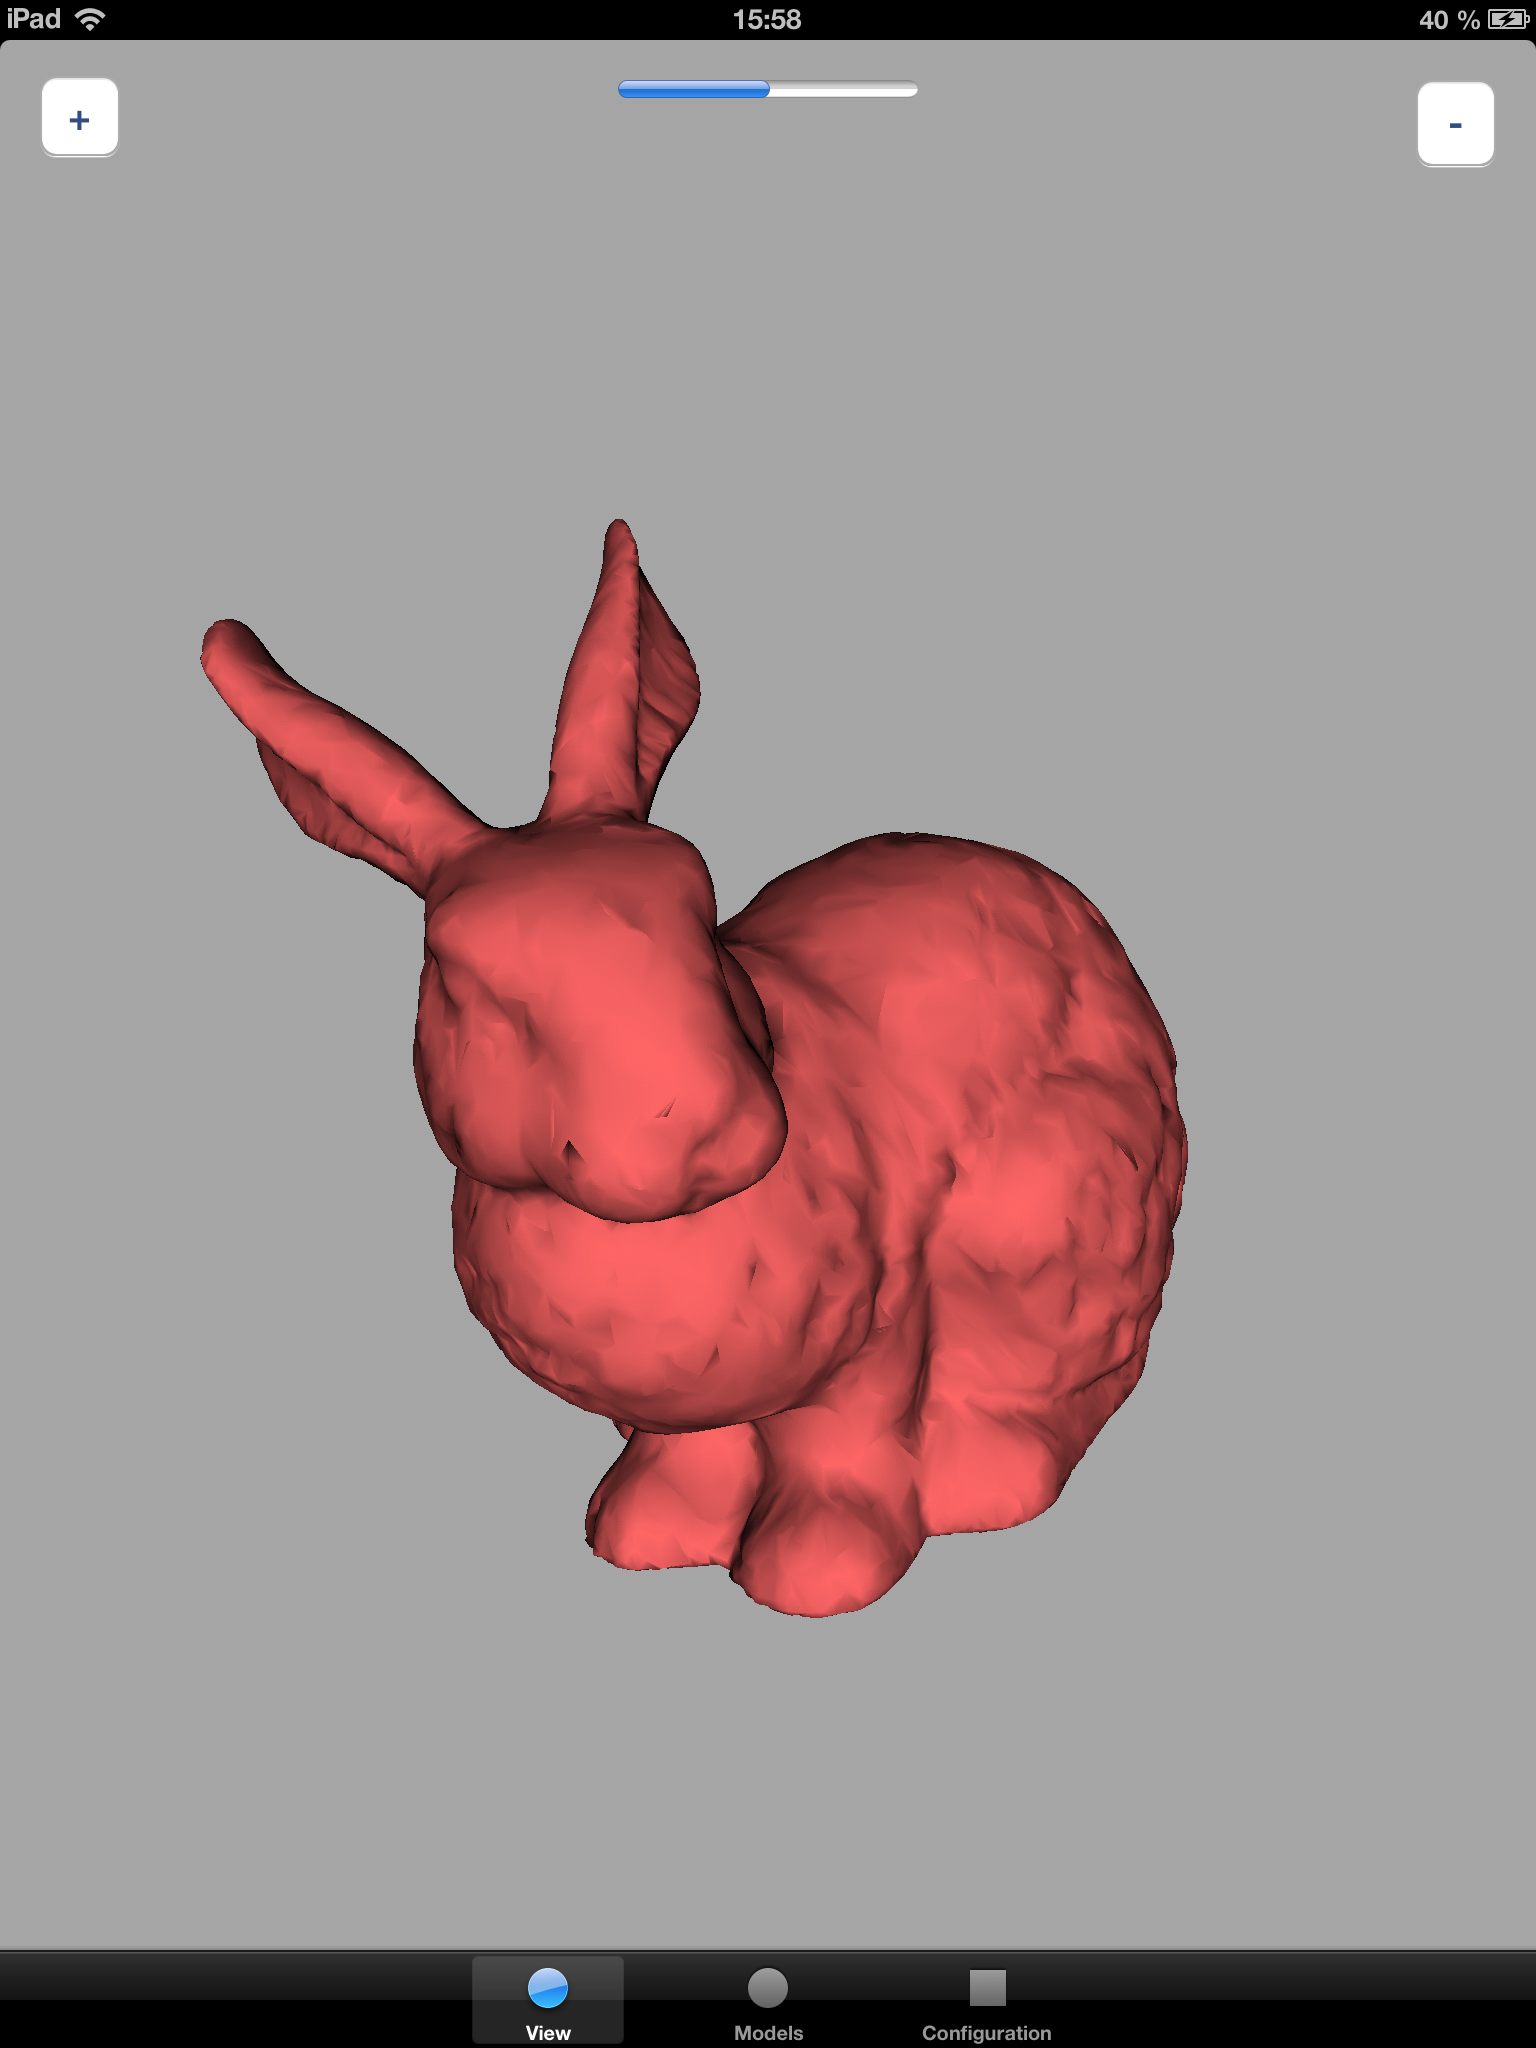
\includegraphics[width=1.0\textwidth]{images/ModelView.png}
	\caption{Screenshot of Model View Tab. There is a status bar on the top of the screen showing refinement process of current LOD}
	\label{fig:modelviewtab}
\end{figure}
\lstinputlisting[label=progmeshglkviewcrtl,caption=ProgMeshGLKViewController.h, style=Xcode, firstline=4, lastline=14]{codes/uiimpl.m}
\FG{fig:modelviewtab} shows the \textbf{Model View} tab of client application on iPad. The Model View tab is implemented using 
\texttt{ProgMeshGLKViewController}, which is subclass of \texttt{GLKViewController} (See Listing~\ref{progmeshglkviewcrtl}). It is mainly responsible for user interaction and rendering the model scene on iPad's screen. 

\subsection{Model List Tab}
\label{section:modellist}
\begin{figure}
	\centering
	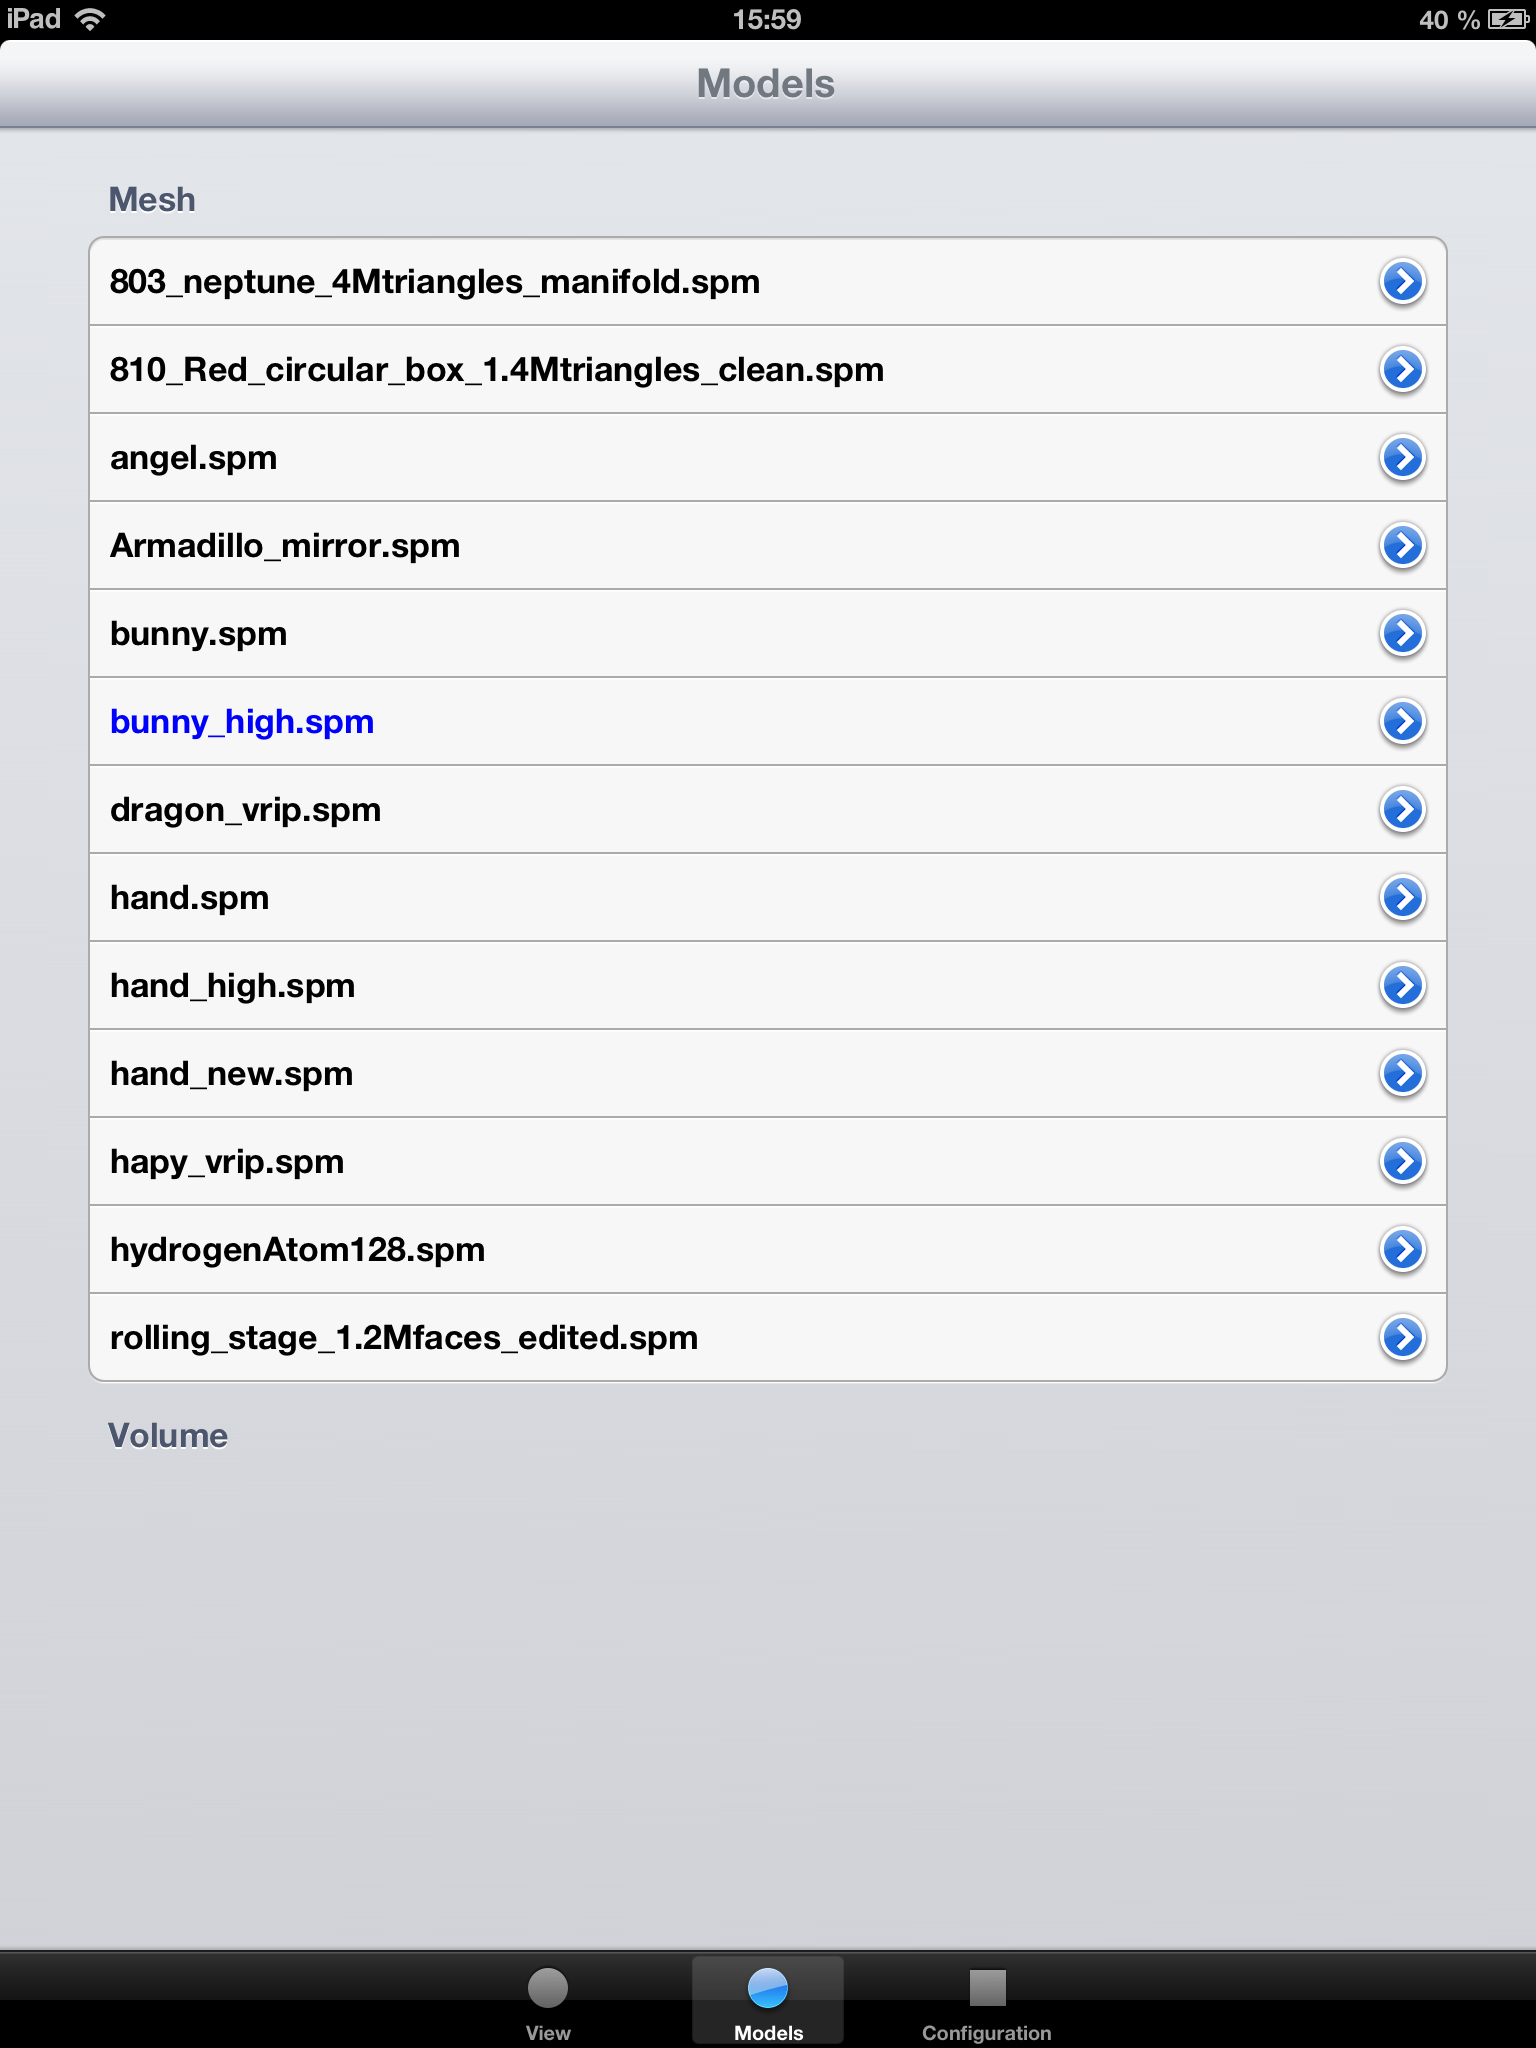
\includegraphics[width=1.0\textwidth]{images/ModelList.png}
	\caption{Screenshot of Model List Tab.}
	\label{fig:modellisttab}
\end{figure}
\lstinputlisting[label=progmeshmodeltableviewctl,caption=ProgMeshModelTableViewController.h, style=Xcode, firstline=17, lastline=24]{codes/uiimpl.m}

The second tab is the \textbf{Model List} tab, as showed in \FG{fig:modellisttab}. It has a list of all currently available models in the mesh repository on the server. When a user picks any item in the list, there will be background thread trying to load the bash mesh of the selected model from server. This tab is implemented using \texttt{ProgMeshModelTableViewController} which extends the base class \texttt{UITableViewController} provided by the iOS system itself (See Listing~\ref{progmeshmodeltableviewctl}). 


\subsection{Configuration Tab}
\label{section:configuration}

\begin{figure}
\centering
\subfigure[b][Configuration tab (disconnected)]{
	\centering
	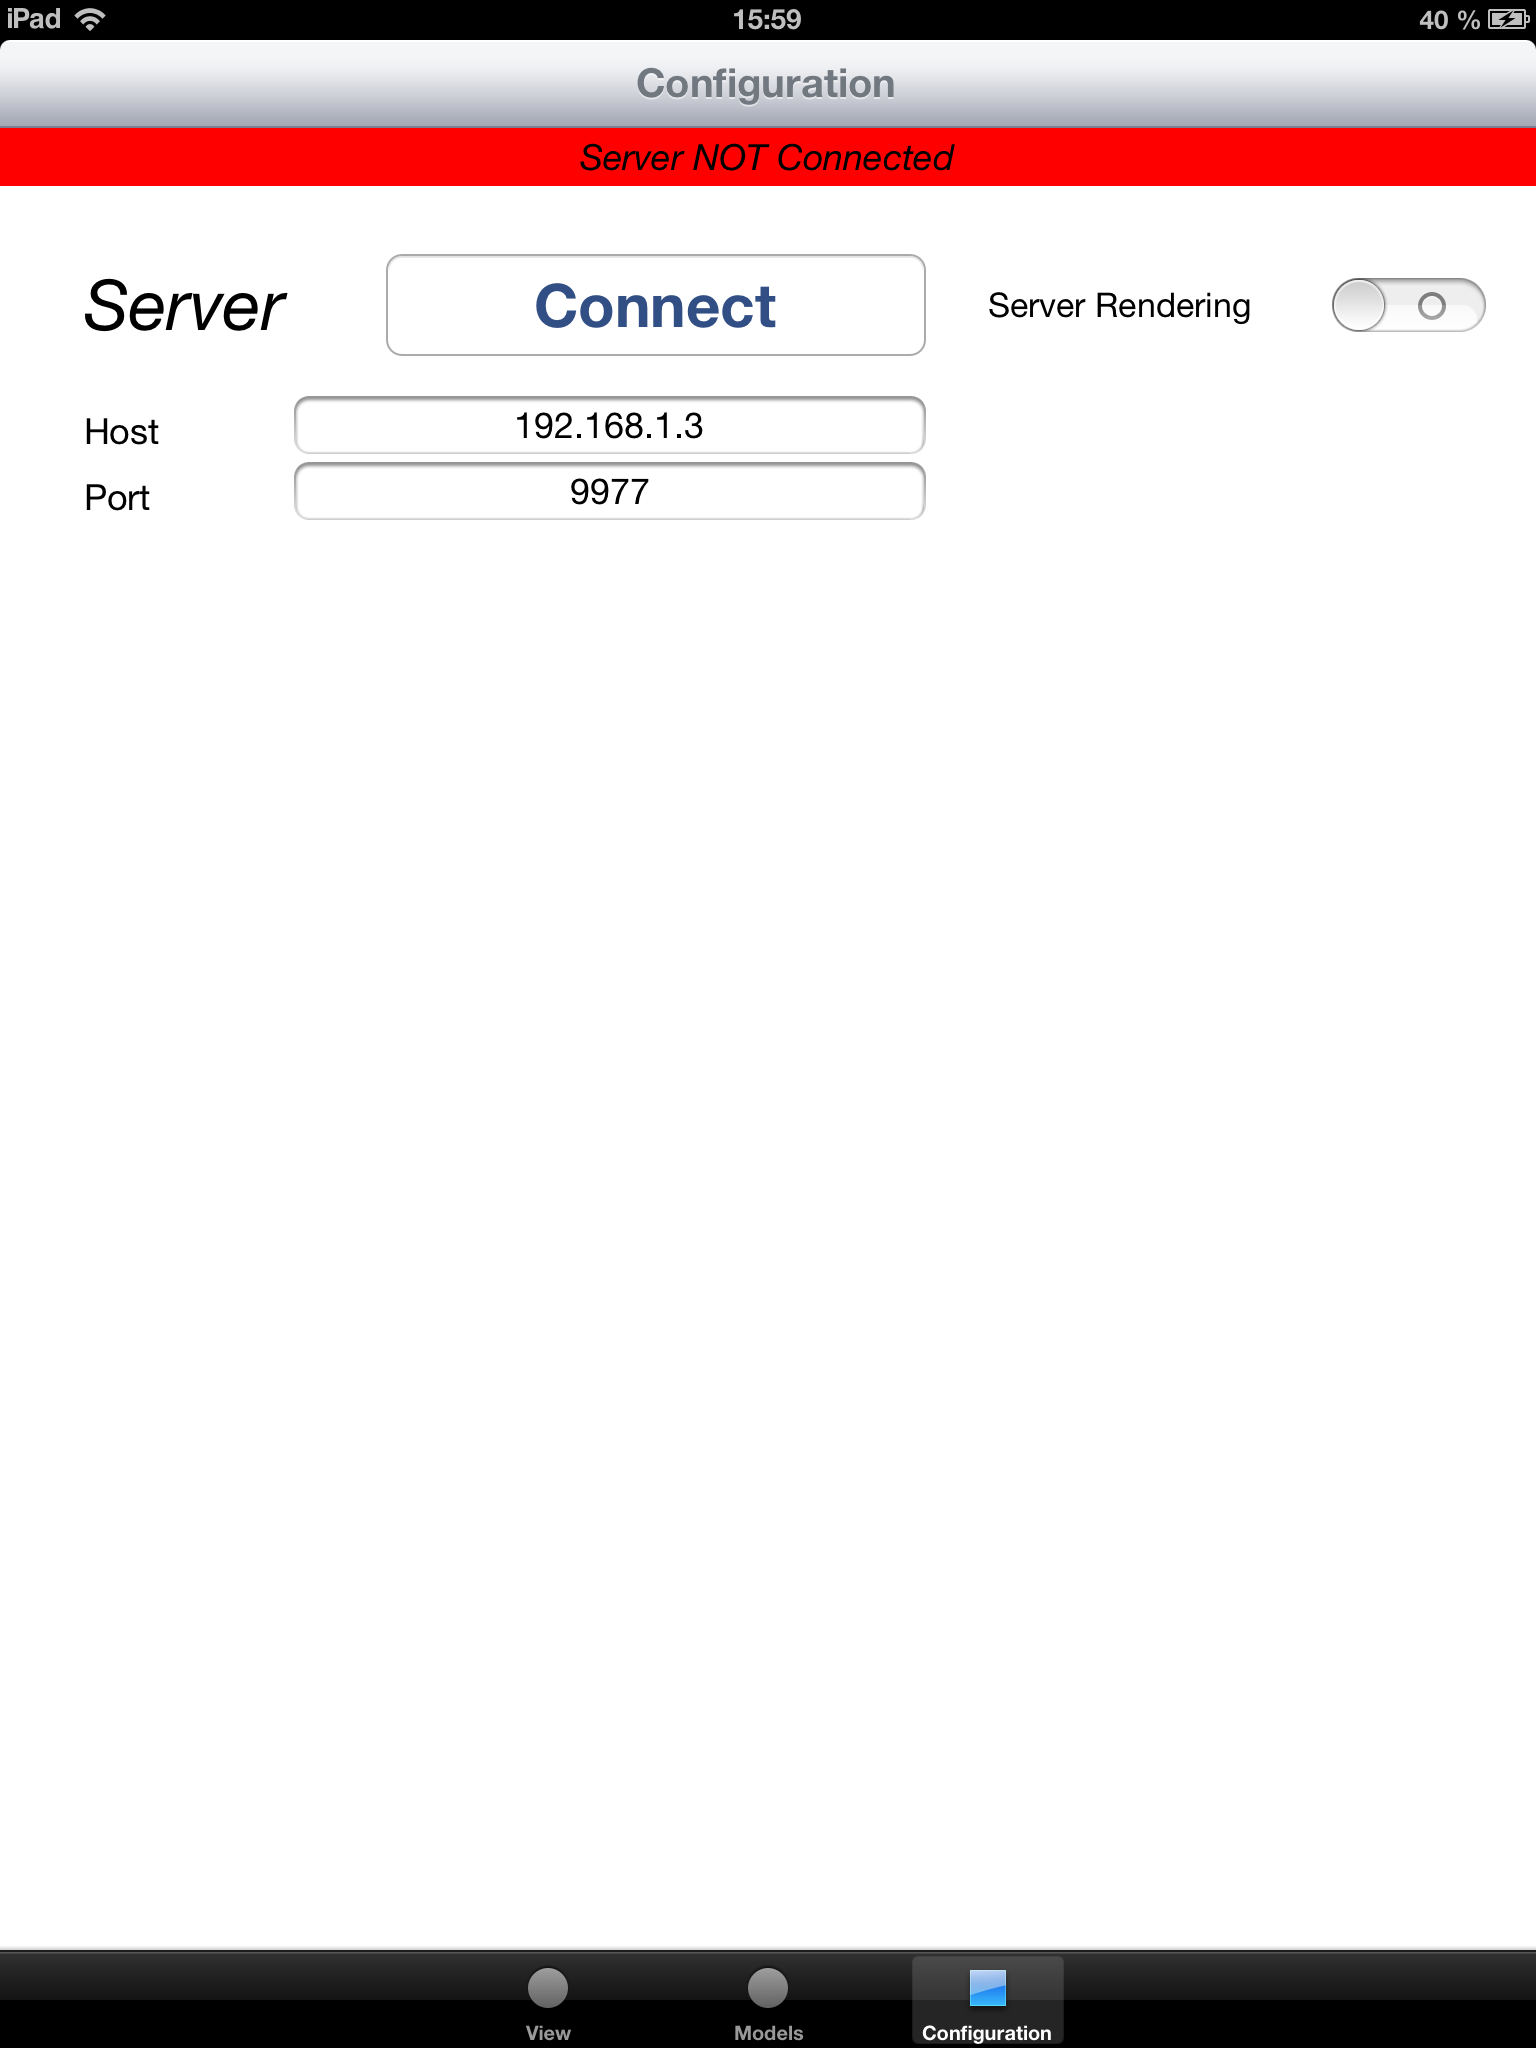
\includegraphics[width =0.45\textwidth] {images/ConfigurationDisconnected.png}
	\label{fig:configtab:disconnected}
}
\hfill
\subfigure[b][Configuration tab (connected)]{
	\centering
	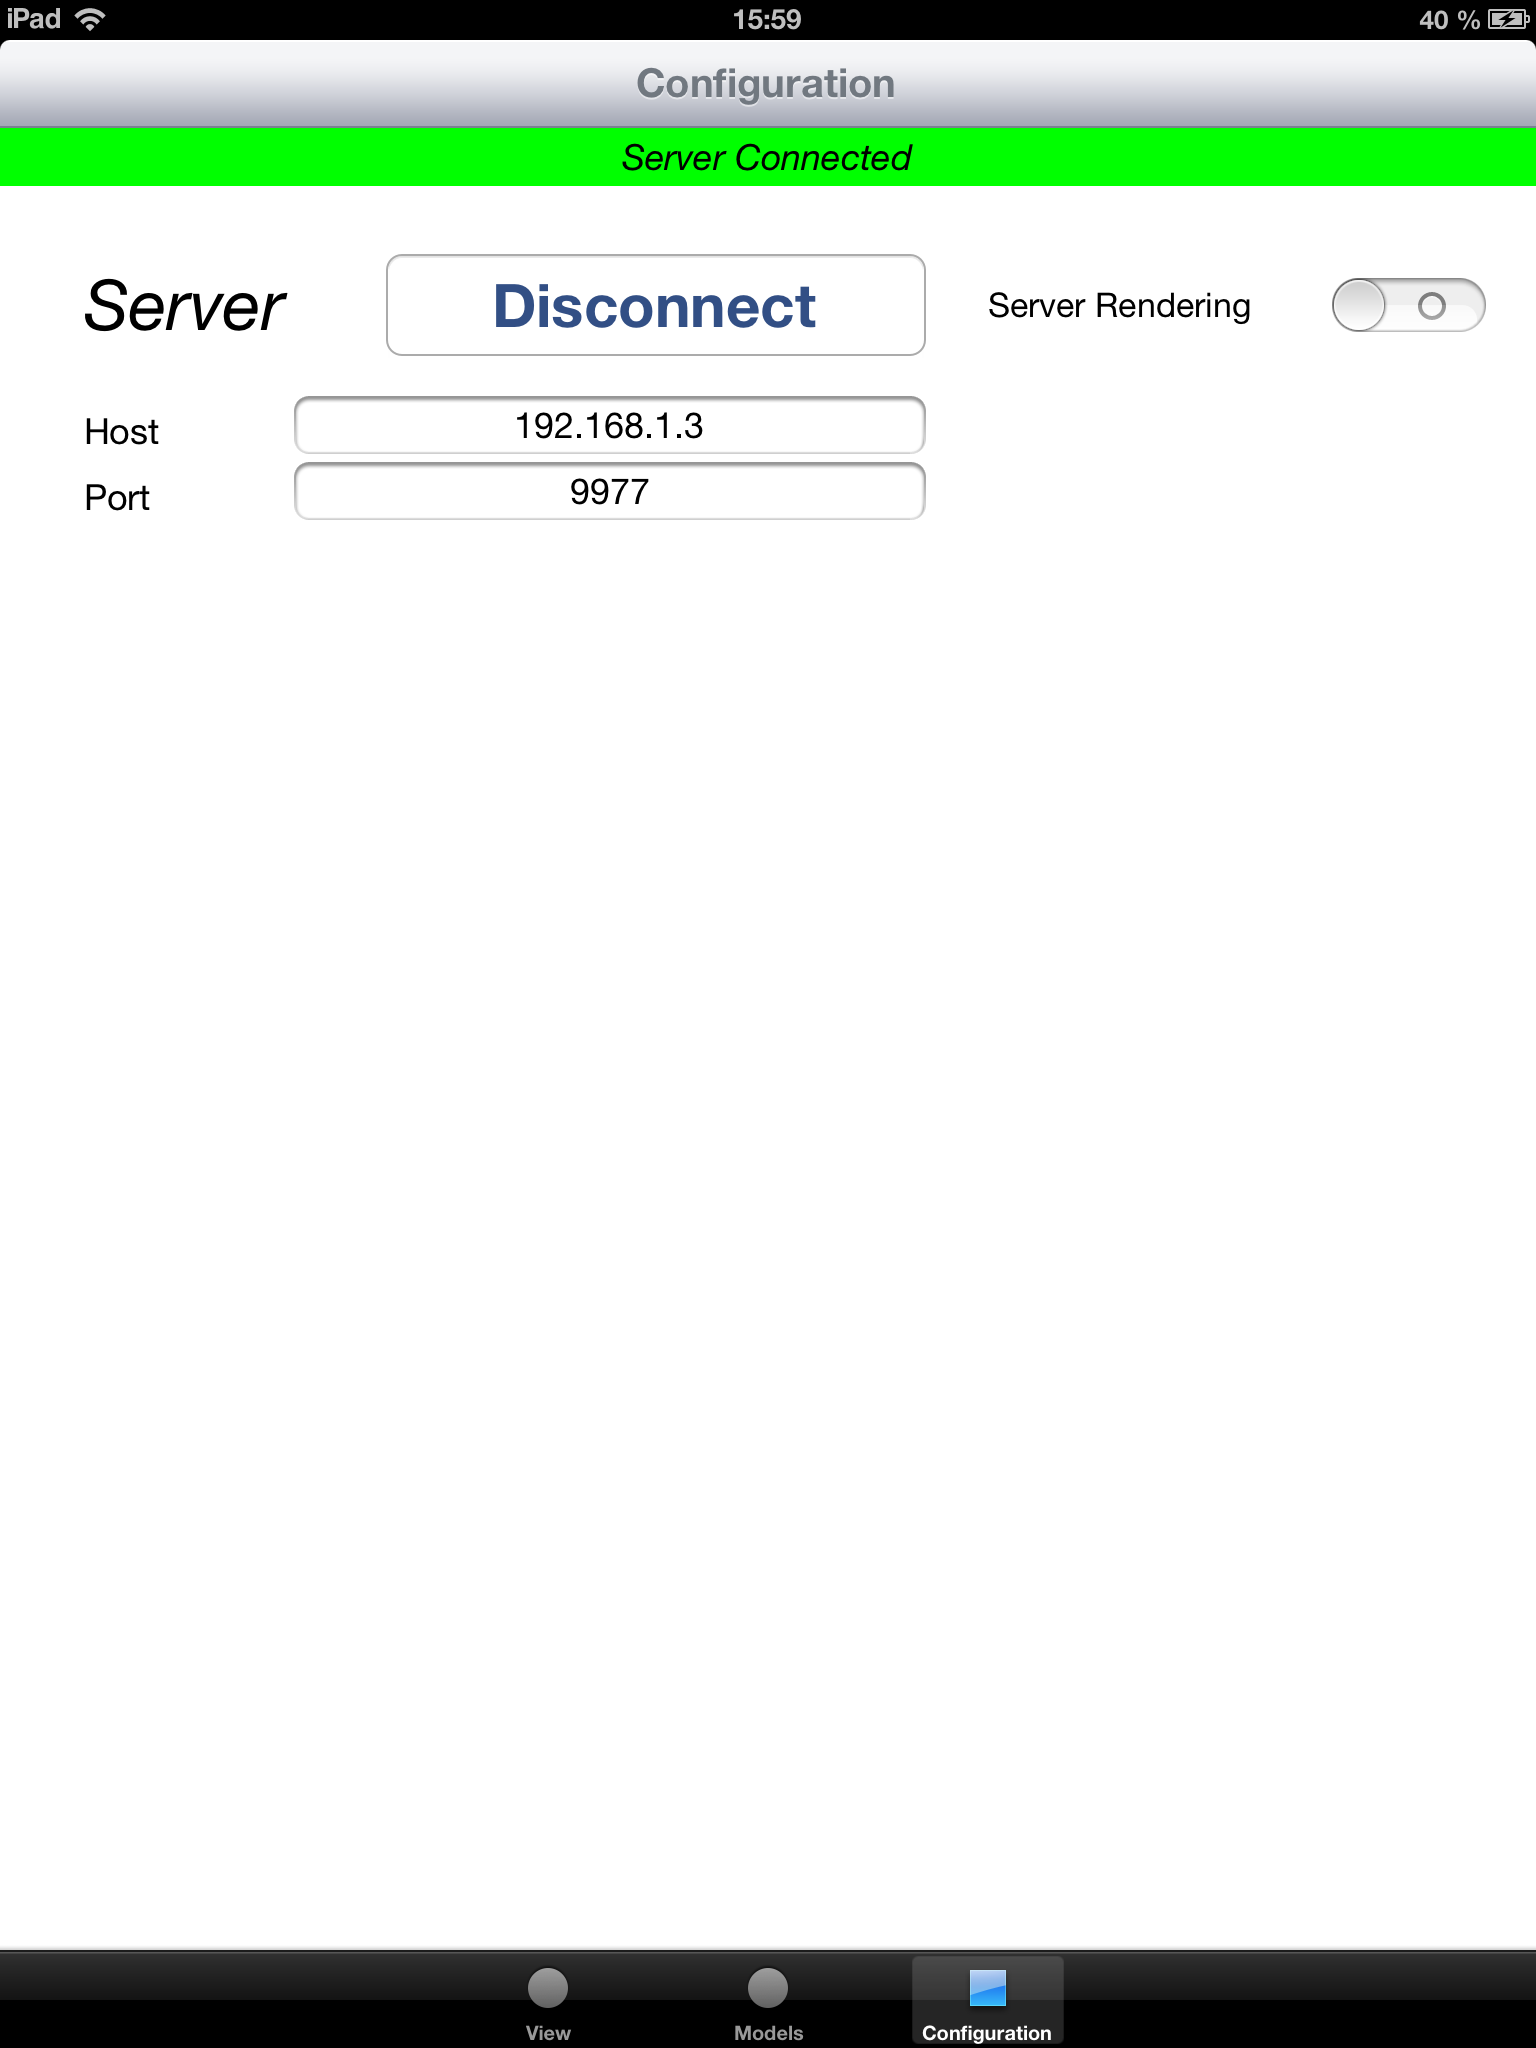
\includegraphics[width =0.45\textwidth] {images/ConfigurationConnected.png}
	\label{fig:configtab:connected}
}
\label{fig:configtab}
\caption{Screenshot of Configuration Tab}
\end{figure}
The last tab, \textbf{Configuration} tab, provides graphics interface to user for the configuration of server IP address, port, control of connection and switching of rendering mode (client/server rendering), as showed in \FG{fig:configtab}. It is implemented using class \texttt{ConfigViewController} which is a subclass of \texttt{UIViewController} (See Listing~\ref{configviewcode}). \\

\noindent
\begin{minipage}{\linewidth}
\makebox[\linewidth]{
\lstinputlisting[label=configviewcode,caption=ConfigViewController.h, style=Xcode, firstline=27, lastline=37]{codes/uiimpl.m}
}
\bigskip
\end{minipage}


%\section{Implementation Discussion}
%\TODO{Discussion on implementation. }

%Picture
%\noindent
%\begin{minipage}{\linewidth}
%\makebox[\linewidth]{%
%\includegraphics[width=1.0\textwidth]{images/morphable.pdf}}
%\captionof{figure}{MorphableUI generates user-tailored interfaces for arbitrary applications in arbitrary environments. Users are able to use all available devices to control as many applications as needed. User behavior is analyzed by the system to increase the user experience.}% only if needed
%\label{fig:morphable}
%\bigskip
%\end{minipage}


